\documentclass[11pt]{article}

\usepackage{listings}
\usepackage{graphicx}
\usepackage{titling}
\usepackage{fullpage}
\newcommand{\subtitle}[1]{%
  \posttitle{%
    \par\end{center}
    \begin{center}\large#1\end{center}
    \vskip0.5em}%
}

%%\renewcommand{\topfraction}{0.9}    % max fraction of floats at top
%%\renewcommand{\bottomfraction}{0.8}

\begin{document}

\title{Deeva}
\subtitle{Planing Report}
\author{Kritaphat Sonsri-in, Xueqi Chen, Hector Dearman, \\Alina Draganescu, Felix De Souza}

\maketitle

\section{The Task}
Our group was assigned to the Project Java Debugger which will be designed for first year computing students. After we discussed with Tristan, who proposed this project, we understood that the problem while teaching Java to first year students is that students tend to get really dependant on IDE like Eclipse with functionalities like auto-fill etc. Tristan has tried alternatives like using JDB however it sometimes gets out of sync and breaks. This is why he wants a simpler version of IDE that is more light-weighted. 

\section{How we prepared the Plan}

\section{Additional Notes}
Was this.

\section{Requirement Analysis}
We had an internal meeting, firstly, to identify stakeholders which involve first year students; Tristan, our project owner; lab helpers; and CSG, who will deploy our project to lab machines. Then, we discussed and shared common understanding of the project. We initialised a list of requirements and did research on debuggers to see the already-exist features. Subsequently, we made an appointment with Tristan to discuss our approach on the project. Regarding the meeting with Tristan, we agreed on our requirements, and Tristan prioritised the features of the debugger. Then we came up with a release plan. Also, we interviewed the students to find out what kind of Java debugger they have used, pros and cons of each one of them and what else they would like to see in the debugger. It appeared that visualization was the most desired feature. In addition, we also considered use cases. After the requirement gathering step, we had a second meeting with Tristan to make a clear final decision concerning core requirements and feature priorities. And, we used contract-style requirement list to provide a contract between us.
Any change made in the plan and requirements were recorded and updated using Google Drive. Major changes were made after the first meeting with Tristan; only slight change was made after the second meeting. 

\section{Agile Programming}
After our first meeting with Tristan, we had our first formal group meeting with the information Tristan had provided us. We decided to use Agile Programming as we go along. A Trello board was then created for a better project management process. There are several different swimlanes on the board: ‘Proposed’, which allows all members to throw in ideas; ‘In analysis’, where people talk about their ideas and have a discussion with group members to see if the story is feasible. If it is, the card will be then moved to ‘In estimation’ where we gather together to use planning pokers to give a complexity points to the story. Otherwise, the story will be moved to ‘Discarded’. The reason why we want to keep track of what we have discarded is that we might have thought we would not have time for it but in reality we did have time at the end, we might want to move it back and reconsider it. One of our group members had hand-made a set of pokers just for estimation. It contains Fibonacci number 0 - 13 and ‘infinity’ if we think it’s impossible to do as well as ‘coffee time’ if we think we need a break. After estimation, the card will be assigned to group members with a set due date and be moved into ‘In development’. Once the development is complete, the card should be moved into ‘In review’. This is when we need someone to review our code to improve our styling and pattern-usage. During the meeting, we came up with some research topics that were neccessary for the project such as: tools/frameworks, different java debugger comparison, getting first year java projects and etc. Everyone picked one story base on their preference with a set deadline. For example, Krit and Kira were working on the comparison of different debuggers, we used google docs for editing and gathering information that we had found. Hector and Felix were working on researching on frameworks. Alina was assigned with making estimation pokers and getting the first year java projects. 

In the next meeting, we tell everyone what we had found and our comments and thoughts in turns.

\section{Our Plan}

\section{Tools}


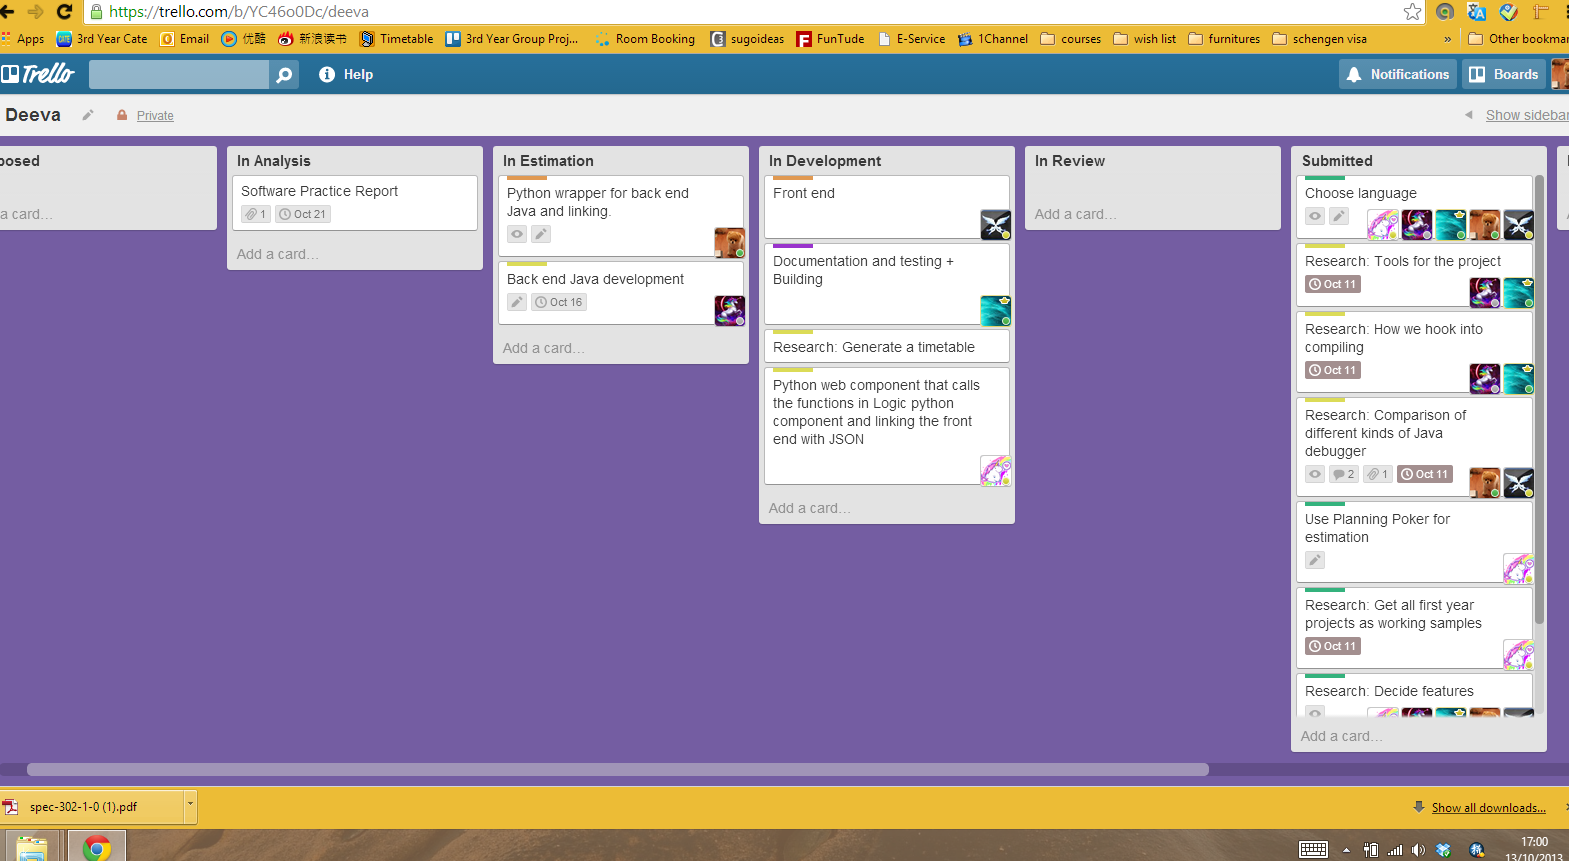
\includegraphics[width=\textwidth]{TrelloBoard.png}

\end{document}
